\documentclass[twocolumn,
amssymb,prb,aps,superscriptaddress]{revtex4}

\usepackage{graphicx}
\usepackage[utf8]{inputenc}
\usepackage{float}

\usepackage{amsmath}
\usepackage{amssymb}
\usepackage{amsthm}
\usepackage{amsfonts}
\usepackage{braket}


\begin{document}

\begin{abstract}
    Hola Abstract, este es un pequeño resumen del documento presentado
\end{abstract}

\title{Resonancia Paramagnetica Spin Electrón}
\author{Majo}

\affiliation{Colegio de Ciencias e Ingeniería, USFQ, Quito, Ecuador} 

\author{Martin}

\affiliation{Colegio de Ciencias e Ingeniería, USFQ, Quito, Ecuador}

\date{\today}

\maketitle

\section[Intro]{Introducción}
\label{sec:intro}

Lo que es, de donde sale, quien lo descubrio, lo que dice en wikipedia y que vamos a decir en paper

\section[]{Cuántica del Sistema}
\label{sec:cuantica}

\subsection{Prototipo Hamiltoniano}

El prototipo basico de RPE es una interaccion entre 2 particulas de Spin $1/2$, el proton del nucleo con spin $\vec{I}$ y el del $e^-$ $\vec{S}$. El hamiltoniano del sistema electron nucleo puede escribirse con terminos de la interacción entre los 2 spines $ \vec{I} \cdot \vec{S} $ y los terminos de Zeeman $g \beta \vec{H} \cdot \vec{J}$, si asumimos que el $\vec{H}$ esta en $z$ tenemos

\begin{equation}
    \label{eq:hamiltonianoDelSistema}
    \mathcal{\hat{H}} = H (g_e \beta \hat{S_z} - g_N \beta_N \hat{I_z}) + T \vec{S} \cdot \vec{I} 
\end{equation}

\subsection{Prototipo Solución}

Para la solución vamos a usar la base de spin nucleo y electron acoplada $\hat{\vec{J}} = \hat{\vec{S}} + \hat{\vec{L}}$. En el orden $\ket{0,0}$, $\ket{1,-1}$, $\ket{1,0}$, $\ket{1,+1}$. En esta base y usando el hecho que $ 2 \hat{\vec{I}} \cdot \hat{\vec{S}} = \hat{J^2} - \hat{S^2} - \hat{I^2} $ tenemos la matriz de $\mathcal{\hat{H}}$

\begin{equation}
    \label{eq:matrizHamiltoniano}
    \hat{\mathcal{H}} =     
\begin{pmatrix}

    -\frac{3}{2} T \hbar^2 & 0 & - \frac{H \hbar}{2} g_+ & 0 \\

    0 & -\frac{H \hbar}{2} g_- + \frac{T \hbar^2}{4} & 0 & 0 \\

    - \frac{H \hbar}{2} g_+ & 0 & \frac{T \hbar^2}{4} & 0 \\

    0 & 0 & 0 & \frac{H \hbar}{2} g_- + \frac{T \hbar^2}{4} \\

\end{pmatrix}
\end{equation}

donde

\begin{align}
    \label{eq:notacionG}
    g_+ = g_e \beta_e + g_N \beta_N \\
    g_- = g_e \beta_e - g_N \beta_N    
\end{align}

\subsection{Energias posibles del Sistema}


Con esta matriz en la base que hemos escogido poedemos diagonalizar, de esta forma tenemos las energias posibles del sistema o los valores propios de la matriz (\ref{eq:matrizHamiltoniano})
%\begin{equation}
    \begin{align*}
        E_1 = \frac{\hbar}{4}(T \hbar - 2 H (g_e \beta_e - g_N \beta_N)) \\
        E_2 = \frac{\hbar}{4}(T \hbar + 2 H (g_e \beta_e - g_N \beta_N)) \\
        E_3 = \frac{\hbar}{8}\left(-5 T \hbar - \sqrt{\frac{8^2 H^2}{2^2} (g_e \beta_e + g_N \beta_N)^2 + 7^2 T^2 \hbar^2}\right) \\
        E_4 = \frac{\hbar}{8}\left(-5 T \hbar + \sqrt{\frac{8^2 H^2}{2^2} (g_e \beta_e + g_N \beta_N)^2 + 7^2 T^2 \hbar^2} \right) \\
    \end{align*}
%\end{equation}
Estas energias si bien son exactas son impracticas para trabajar, comunmente en la resonancia paramagnetica electronica se cumple que 

\begin{equation}
    \label{eq:aproximacion}
    (g_e \beta_e + g_N \beta_N)^2 H^2 >> T^2 \hbar^2    
\end{equation}

 Vamos a usar esta aproximación y los primeros 2 terminos de la seria $ \sqrt{1 + \epsilon^2} = 1+\frac{\epsilon^2}{2}-\frac{\epsilon^4}{8} + ... $ con $ \epsilon = \frac{7}{4}\frac{T \hbar}{H(g_e \beta_e + g_N \beta_N)} $ entonces el termino de la raiz se aproxima a
$$ 4 H (g_e \beta_e + g_N \beta_N) \times \left(1 + \frac{7^2}{2 \times 4^2} \frac{T^2 \hbar^2}{H^2(g_e \beta_e + g_N \beta_N)^2} \right) $$ 
con el error dependiendo de $\epsilon^4$
Las energias resultantes tenemos

\begin{equation}
    \label{eq:energia1}
    E_1 = \frac{\hbar}{4}(T \hbar - 2 H g_-)
\end{equation}

\begin{equation}
    \label{eq:energia2}
    E_2 = \frac{\hbar}{4}(T \hbar + 2 H g_-)
\end{equation}

\begin{equation}
    \label{eq:energia3}
    E_3 \approx -\frac{5}{8} T \hbar^2 - \frac{H \hbar}{2} g_+ - \frac{7^2}{8^2} \frac{T^2 \hbar^2}{Hg_+}
\end{equation}

\begin{equation}
    \label{eq:energia4}
    E_4 \approx -\frac{5}{8} T \hbar^2 + \frac{H \hbar}{2} g_+ + \frac{7^2}{8^2} \frac{T^2 \hbar^2}{Hg_+}
\end{equation}

donde nuevamente hemos usando la notación de (\ref{eq:notacionG})

Ahora vamos a mostrar como dependen las energias del campo magnetico. 


    \begin{figure}[H]
        \centering
        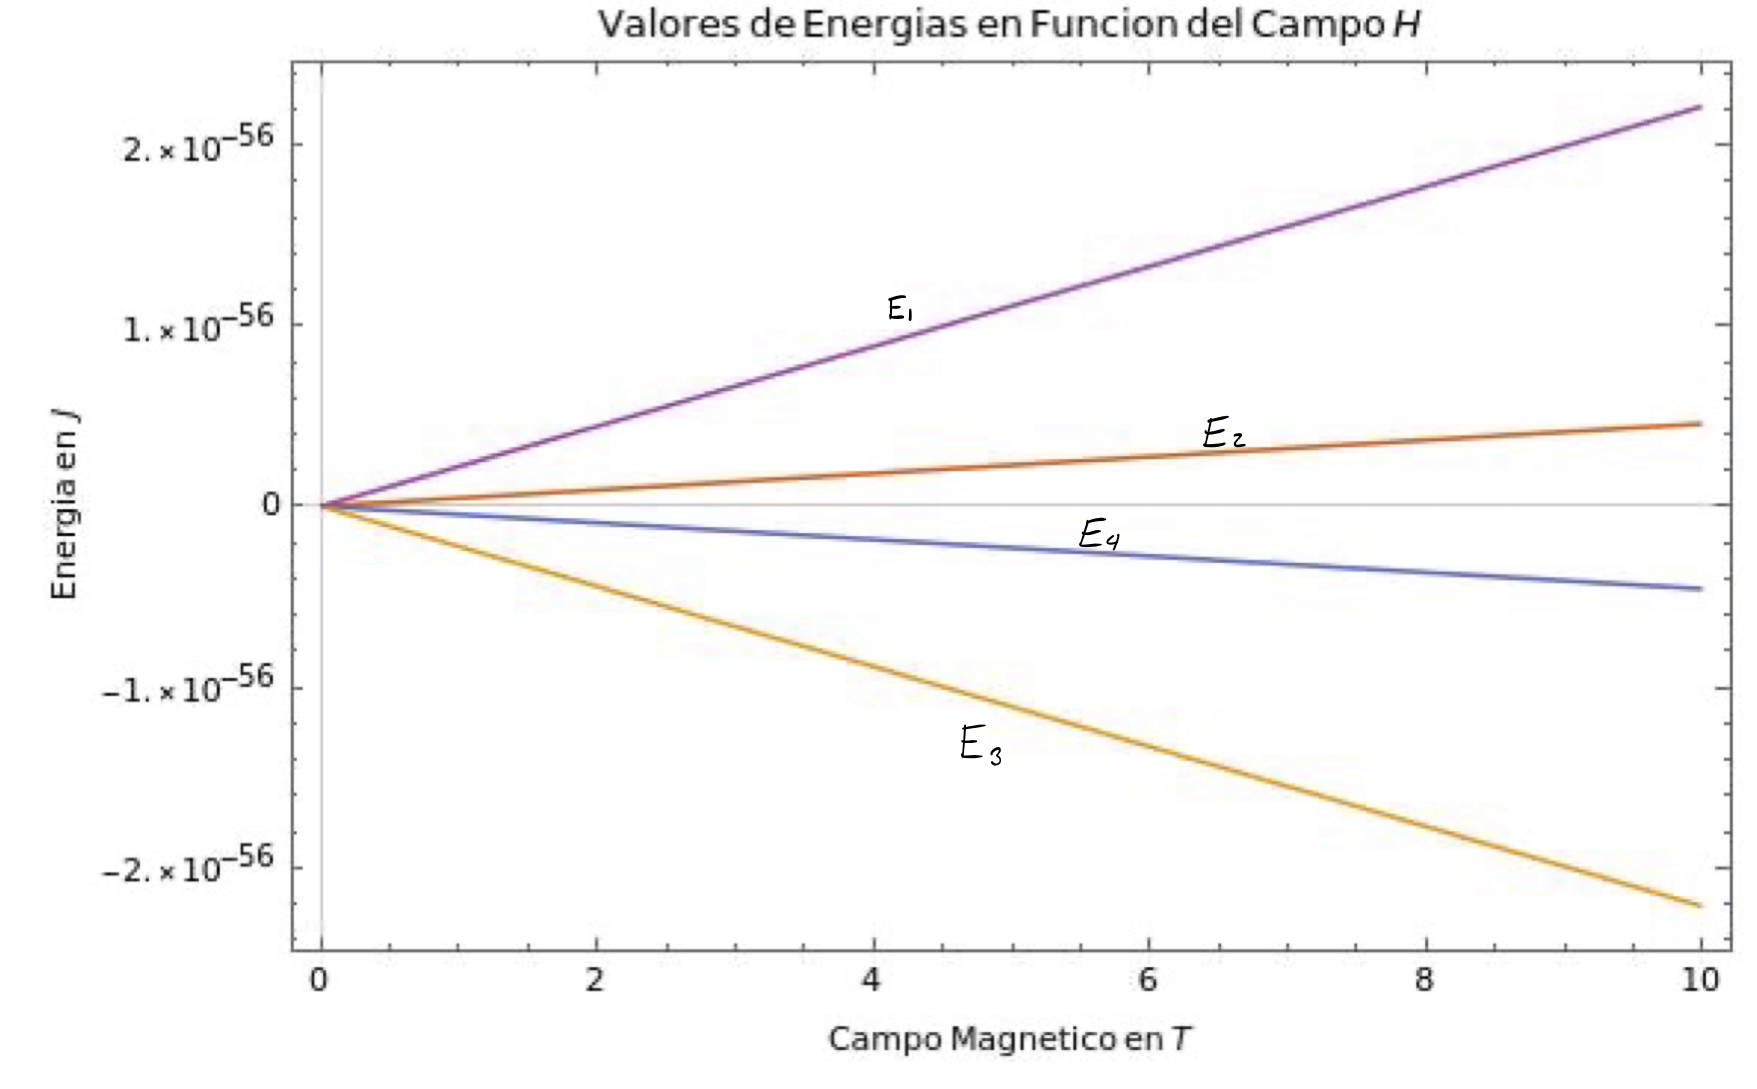
\includegraphics[width=7cm]{images/GraficoEnergiasCamp.jpg}
        \caption{Posibles Valores de Energia en Función del Campo H}
        \label{fig:diagramaDeEnergia}
    \end{figure}

    Podemos agrupar las energias $E_1$ con $E_2$ como las energias positivas y $E_3$ con $E_4$ como las negativas. Los saltos de energia para variar el spin entre $E_3$ y $E_1$ y entre $E_4$ y $E_2$. De esta forma los saltos de energia serian $\Delta E_{13} = E_1 - E_3$ y $\Delta E_{24} = E_2 - E_4$ ya que tenemos que movernos entre las energias positivas y las negativas para tener fenomenos de resonancia.

    \begin{equation}
        \Delta E_{13} = \frac{\hbar}{64} \left(-32 \hbar g_- +\frac{49 h T^2}{g_+ H}+32 g_+ H+56 h T\right)
    \end{equation}

    \begin{equation}
        \Delta E_{24} = \frac{\hbar}{64} \left(32 \hbar g_- -\frac{49 h T^2}{g_+ H}-32 g_+ H+56 h T\right)
    \end{equation}

    \subsection{Kets Propios del Hamiltoniano}

    Como los kets $\ket{1,-1} = \ket{--}$ y el $\ket{1,1} = \ket{++}$ estos son vectores propios de $\hat{S_z}$, $ \hat{I_z}$, $ \hat{S^2}$, $ \hat{I^2}$ $ \hat{J^2}$ por ende tambien lo son del Hamiltoniano. En lugar de resolver las ecuaciones para los otros 2 vamos a proponer solucion de la forma 
    $$ \ket{E3} = \alpha \ket{0,0} + \omega \ket{1,1} $$ 
    el otro es ortogonal a los anteriores es decir 
    $$ \ket{E4} = -\omega \ket{0,0} + \alpha \ket{1,1} $$

    con estas condiciones vamos a tener un $\alpha$ y un $\omega$ no normalizados, normalizaremos el vector despues de aplicar la aproximación (\ref{eq:aproximacion}).

    \begin{equation}
        \alpha = 7 \hbar T+\sqrt{16 g_+^2 H^2+49 \hbar^2 T^2}
    \end{equation}
    \begin{equation}
        \omega = -4g_+ H
    \end{equation}
    
    vamos a usar el mismo truco que usamos para obtener las ecuaciones (\ref{eq:energia3}) y (\ref{eq:energia4}) solo que el epsilon ahora es $ 7 \hbar T / (4 g_+ H) $ de donde tenemos 

    \begin{equation*}
       \alpha = 7 \hbar T + 4 g_+ H + \frac{(7 \hbar T)^2}{8 g_+ h}
    \end{equation*}

     si bien este $\alpha$ tiene error $O(\epsilon^2)$ lo que se trabaja con estos vectores propios requiere conocimiento de teoria de perturbaciones para potenciales dependentes del tiempo. Dado que cuando los fotones ingresan al campo magnetico la energia de estos y como afectan varia el tiempo. Por esta razon vamos a presentar los vectores propios solo con los primeros 2 terminos de $\alpha$

    Tenemos entonces que 
    \begin{equation}
        \ket{E_3} = \frac{1}{\gamma} [(7 \hbar T + 4 g_+ H) \ket{0,0} - 4 g_+ H \ket{1,1}]
    \end{equation}
    \begin{equation}
        \ket{E_4} = \frac{1}{\gamma}  [4 g_+ H \ket{0,0} + (7 \hbar T + 4 g_+ H) \ket{1,1}]
    \end{equation}

    donde 
    \begin{equation*}
        \gamma = \sqrt{(7 \hbar T)^2 + 2 (4 g_+ H)^2 + 56 \hbar T g_+ H}
    \end{equation*}
    
\end{document}